\section{مقدمه}
در فصل‌های قبل روش طراحی منطق دامنه بر اساس تبادل ناهمگام پیغام ارائه شد و برخی از الگوهای طراحی در این روش به همراه نکات مهم آن مورد بررسی قرار گرفت. در این فصل دو معیار کیفی تغییرپذیری و کارایی در طراحی به این روش مورد ارزیابی قرار می‌گیرد. برای انجام ارزیابی ابتدا سیستم معرفی شده در بخش \ref{section:eduIntro} بر اساس طراحی ارائه شده، پیاده سازی شده است. با توجه به اینکه قضاوت در مورد معیارهای انتخاب شده برای بررسی، در مقایسه با رویکرد طراحی شیءگرا مفهوم پیدا می‌کند سیستم مذکور توسط روش متداول شیءگرا نیز طراحی و پیاده‌سازی شده است. در پیاده‌سازی نسخه‌ی شیءگرا از الگوی مدل دامنه \cite{Fowler_Patterns} برای لایه‌ی منطق دامنه بهره گرفته شده است. ضمناً به هدف نزدیکتر شدن سیستم معرفی شده به پیاده‌سازی‌های واقعی، امکان ماندگاری\LTRfootnote{persistence} داده‌ها در پایگاه داده نیز به هر دو طراحی افزوده گردیده است. در هر دو پیاده‌سازی از الگوی \gls{مخزن}\LTRfootnote{repository}\cite{Fowler_Patterns} برای نگاشت اشیاء دامنه به جداول پایگاه داده استفاده شده است.
با توجه به حجم بالای برنامه‌های پیاده‌سازی شده و نیز به هدف قابلیت استفاده‌، متن برنامه‌ی تولید شده به هر دو روش به همراه کتابخانه‌های لازم برای اجرا، به صورت برخط در دسترس عموم قرار داده شده‌ است\cite{sources_java,sources_scala}. جهت حفظ دقت مقایسه تلاش شده است تا دو طراحی از نظر کارکرد حداکثر شباهت با یکدیگر را داشته باشند. برای پیاده‌سازی سیستم به روش طراحی بر اساس تبادل ناهمگام پیغام، از کتابخانه‌ی اکتور اسکالا استفاده شده و برای پیاده‌سازی به روش شیءگرا از زبان جاوا استفاده شده است. در پایان این قسمت یادآوری می‌شود که تحلیل دقیق و عمیق دلیل اختلاف‌های احتمالی در معیارهای مقایسه شده بین دو روش در حوزه‌ی این پژوهش نیست و هدف از انجام این ارزیابی صرفاً قیاس دو روش از نظر معیارهای انتخاب شده است.
\section{روش ارزیابی}
در این ارزیابی از روش \textit{هدف-پرسش-معیار}\LTRfootnote{Goal-Question-Metric} استفاده شده است. هدف-پرسش-معیار یک روش نظام‌مند برای تعیین معیارهای ارزیابی متناسب با دامنه‌ی مسئله است. این روش یک رویکرد بالا-به-پایین\LTRfootnote{top-down} است که از قدم‌های زیر تشکیل می‌شود:\cite{GQM}
\begin{enumerate}
\item تعیین هدف: به این پرسش پاسخ می‌دهد که \textbf{هدف} از اندازه‌گیری  و ارزیابی چه چیزی است.
\item قدم بعدی تعریف \textbf{پرسش‌}هایی است که اگر پاسخ آنها داده شود هدف اندازه‌گیری برآورده می‌شود.
\item برای پاسخ کمّی به پرسش‌هایی که تعریف شده‌اند، به هر پرسش دسته‌ای از \textbf{معیار}ها تخصیص داده می‌شود.
\end{enumerate}

\begin{figure*}[htb]
    \begin{center}
	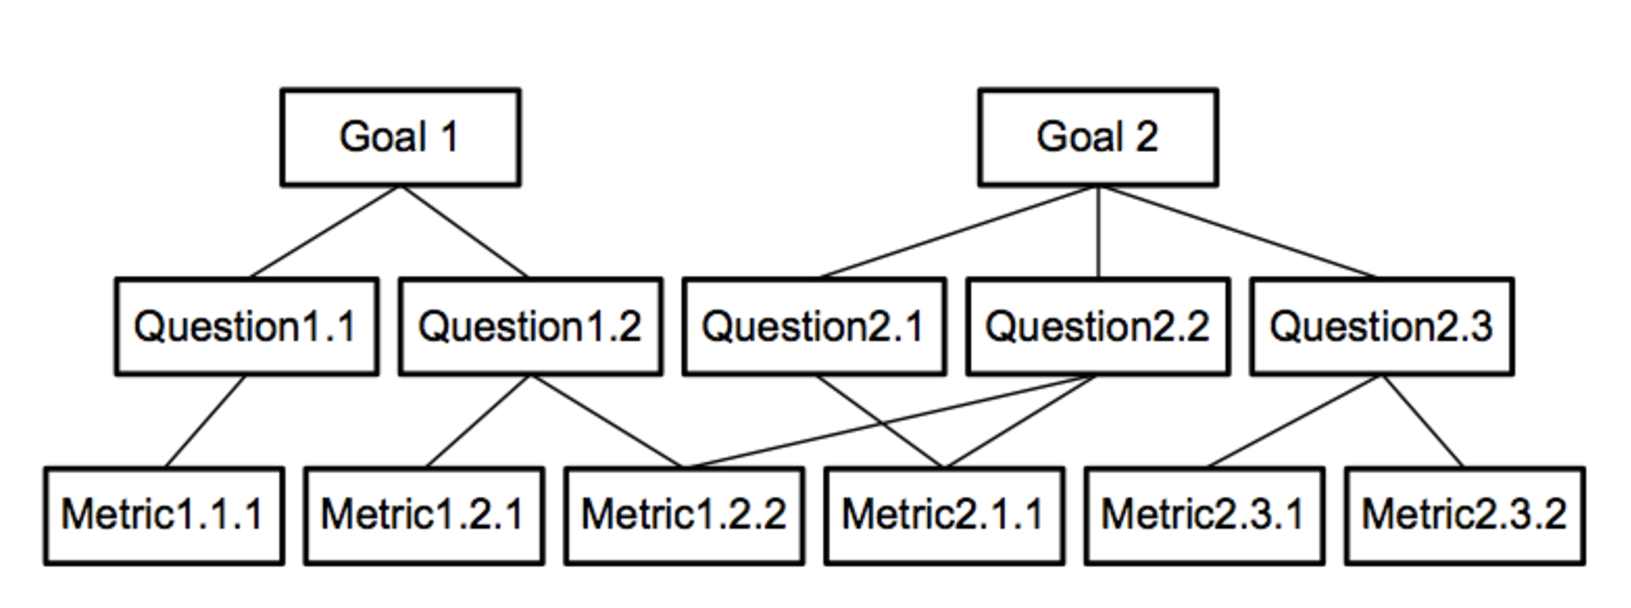
\includegraphics[width=10cm]{5-Evaluation/Figures/gqm.pdf}
    \end{center}
    \caption{\label{fig:gqm} ساختار روش هدف-پرسش-معیار }
\end{figure*}

\section{ارزیابی تغییرپذیری}
در این بخش به ارزیابی تغییرپذیری سیستم تحت طراحی بر اساس تبادل ناهمگام پیغام می‌پردازیم. برای ایجاد امکان ارزیابی کمّی تغییرپذیری، می‌توان از معیارهای کیفیت نرم‌افزار\LTRfootnote{Software Quality Metrics} استفاده کرد. این معیارها خصوصیاتی از قبیل پیچیدگی، قابلیت استفاده‌ی مجدد و آزمون‌پذیری یک سیستم را به صورت کمّی قابل سنجش و مقایسه می‌کنند. در ادامه با توجه به روش هدف-پرسش-معیار، عناصر ارزیابی تغییرپذیری سیستم را تعیین می‌کنیم.

\subsection{هدف}
در این ارزیابی هدف ارزیابی تغییرپذیری طراحی به روش تبادل ناهمگام پیغام است. این ارزیابی از طریق مقایسه‌ی نسخه‌های پیاده سازی شده‌ی سیستم آموزش ساده (بخش \ref{section:eduIntro}) به دو روش طراحی تبادل ناهمگام پیغام و طراحی متداول شیءگرا صورت می‌پذیرد.

\subsection{پرسش‌ها}
برای این ارزیابی ۳ پرسش در نظر گرفته می‌شود:
\begin{enumerate}
\item سیستم طراحی شده به روش تبادل ناهمگام، از نظر معیارهای کیفیت نرم‌افزار چگونه با سیستم طراحی شده به روش شیءگرا مقایسه می‌شود؟
\item اعمال تغییر قواعد منطق برنامه\LTRfootnote{business rules} روی کدام نوع طراحی مشکل‌تر است؟ 
\item اعمال تغییر در مدل دامنه‌ی سیستم روی کدام نوع طراحی مشکل‌تر است؟ 
\end{enumerate}

\subsection{معیارها}
% به منظور پاسخ به هر کدام از پرسش‌های بالا می‌توان از معیارهای کیفیت در برنامه‌نویسی شیءگرا  استفاده کرد. پاسخ به پرسش اول مستقیماً با مقایسه‌ی معیارها پاسخ داده می‌شود. برای پرسش به پاسخ دوم، تغییرات منطق دامنه انتخاب و در هر دو سیستم اعمال می‌شوند و میزان تغییر هر کدام از معیارهای کیفیت بررسی و مقایسه می‌شود. برای پاسخ به پرسش سوم نیز به طریق مشابه می‌توان مقایسه را بعد از اعمال تغییر در مدل دامنه انجام داد. 
در پژوهش‌های مختلف، معیارهای مختلفی برای بررسی کیفیت برنامه‌های شیءگرا ارائه شده‌اند که از آن جمله می‌توان به معیارهای ابریو\LTRfootnote{Abreu}\cite{quality_metrics_1,quality_metrics_2}، معیارهای بانسیا و همکاران\LTRfootnote{Bansia et al}\cite{quality_metrics_3} و معیارهای چیدامبر و کمرر\LTRfootnote{Chidamber and Kemerer} (که به متریک‌های سی‌کِی معروف هستند) اشاره کرد \cite{quality_metrcs_ck}. در این پژوهش تعدادی از متریک‌های موجود برای ارزیابی انتخاب شده‌اند. این انتخاب بر اساس میزان ارجاع در پژوهش‌های مختلف به این متریک‌ها و نیز تناسب آنها با طراحی‌های این پژوهش انجام شده است. مقاله‌ی \cite{metrics_stateOfTheArt} اطلاعات کاملی از متریک‌های مختلف کیفیت نرم‌افزار و میزان ارجاع به آنها را ارائه کرده است. معیارهای انتخاب شده برای پرسش اول، در ادامه معرفی شده‌اند. در تعاریف و توضیحات این معیارها از مقاله‌ی \cite{metrics_stateOfTheArt} بهره گرفته شده است.
\begin{enumerate}
\item\textbf{تعداد کلاس:}
 تعداد کلاس‌های پیاده‌سازی شده (بدون در نظر گرفتن کلاس‌های داخلی)
\item\textbf{میانگین تعداد متد در هر کلاس}

\item\textbf{میانگین تعداد فیلد تعریف شده در هر کلاس}

\item\textbf{تعداد خطوط متن برنامه}

\item\textbf{میانگین تعداد خطوط متن هر کلاس}

\item\textbf{میانگین پیچیدگی چرخه‌ای \lr{(CC)}\LTRfootnote{Average Cyclomatic Complexity}:}
پیچیدگی چرخه‌ای یک متد برابر است با تعداد نقاط تصمیم در گراف کنترل آن بعلاوه‌ی یک. نقاط تصمیم در یک متد در شرط‌ها و حلقه‌ها و دستورهای مشابه رخ می‌دهند. به عنوان مثال، پیچیدگی چرخه‌ای برای یک متد که یک بلوک شرط \lr{(if)} یا یک حلقه دارد عدد ۲ است و برای متدی که صرفاً دستورات خطی دارد عدد ۱ است. هرچه عدد پیچیدگی چرخه‌ای بزرگتر باشد برنامه به موارد آزمون بیشتری نیاز دارد.
\item\textbf{میانگین متدهای وزن‌دار در کلاس\LTRfootnote{Average Weighted Methds per Class}:}
تعداد متدهای وزن‌دار در یک کلاس برابر است با جمع پیچیدگی چرخه‌ای متدهای آن کلاس.
\item\textbf{میانگین عمق درخت وراثت \lr{(DIT)}\LTRfootnote{Average Depth of Inheritance Tree}:}
عمق درخت وراثت برابر است با تعداد کلاس‌هایی که در زنجیره‌ی وراثت یک کلاس آن را به ریشه می‌رساند.

\item\textbf{میانگین تعداد فرزندان:}
تعداد فرزندان یک کلاس برابر است با تعداد کلاس‌هایی که در زنجیره‌ی وراثت کلاس پایین‌تر از خود کلاس هستند.
\item\textbf{میانگین \gls{جفت‌شدگی}\LTRfootnote{Coupling} بین اشیاء:}
یک کلاس با کلاس دیگر جفت‌شدگی دارد اگر یکی از دو کلاس (یا هردو) متدی از دیگری را فراخوانی کرده باشد. معیار جفت‌شدگی بین اشیاء برای یک کلاس برابر است با تعداد کلاس‌های که با کلاس مورد نظر جفت‌شدگی دارد. (معیار انتخاب شده میانگین این عدد در بین همه‌ی کلاس‌ها است.)
\end{enumerate}
پرسش‌های دوم و سوم مربوط به اعمال تغییرات در قواعد منطق دامنه و مدل دامنه‌ی سیستم می‌باشند. برای این پرسش‌ها معیارهای زیر مناسب تشخیص داده شده‌اند:
\begin{enumerate}
\item تعداد خطوط اضافه شده به متن برنامه
\item تعداد کلاس اضافه شده
\item تعداد متد وزن‌دار اضافه شده
\item تعداد کلاس تغییر داده شده
\item تعداد متد تغییر داده شده
\end{enumerate}
\subsection{نتایج ارزیابی}
\subsubsection{پرسش اول}
برای پاسخ به پرسش اول، معیارهای انتخاب شده در پیاده‌سازی‌های سیستم آموزش ساده (بخش \ref{section:eduIntro}) به دو روش تبادل ناهمگام پیغام و شیءگرا محاسبه شده و باهم مقایسه شده‌اند. نتیجه‌ی این مقایسه در جدول \ref{table:mod_result_1} ارائه شده است.


%%%%%%%%%%%%%%%%%%%%%%%%%%%%%
%%%%  Q1 results
%%%%%%%%%%%%%%%%%%%%%%%%%%%%%
\begin{table}[ht]
\small
\begin{center}
\begin{tabular}{|p{7cm}|p{4cm}|p{4cm}|}
	\hline
%	\multicolumn{1}{|p{7cm}}{Header 1} & \multicolumn{1}{p{4cm}}{Header 2} & \multicolumn{1}{p{4cm}|}{Header 3} \\
%\multicolumn{1}{|p{7cm}}{\textbf{معیار}} & \multicolumn{1}{|p{4cm}}{\textbf{مقدار معیار برای طراحی به روش شیءگرا}} & \multicolumn{1}{|p{4cm}|}{\textbf{مقدار معیار برای طراحی به روش تبادل ناهمگام پیغام}} \\
\textbf{معیار} & \textbf{مقدار معیار برای طراحی به روش شیءگرا} & \textbf{مقدار معیار برای طراحی به روش تبادل ناهمگام پیغام} 
\\ 
	\hline
	تعداد کلاس
	 &
	 ۱۵
	 &
 ۱۷
\\
	\hline
	میانگین تعداد متد در هر کلاس
	 &
	 ۶/۲
	 &
	 ۵/۱۱
\\
	\hline
	میانگین تعداد فیلد تعریف شده در هر کلاس
	 &
	 ۱/۹۳
	 &
	 ۲/۱۴
\\
	\hline

	تعداد خطوط متن برنامه
	 &
	 ۶۶۴
	 &
	 ۷۶۰
\\
	\hline
	
		میانگین تعداد خطوط متن هر کلاس
	 &
	 ۴۴/۲۷
	 &
	 ۴۲/۲۲
\\
	\hline
	
		میانگین پیچیدگی چرخه‌ای
	 &
	 ۱/۵۸
	 &
	 ۱/۲۵
\\
	\hline
	
		میانگین متدهای وزن‌دار در کلاس
	 &
	 ۹/۸
	 &
	 ۷/۱۲
\\
	\hline
	
		میانگین عمق درخت وراثت
	 &
	 ۱/۳۳
	 &
	 ۱/۵۹
\\
	\hline
	
		میانگین تعداد فرزندان
	 &
	 ۰/۳۳
	 &
	 ۰/۵۹
\\
	\hline
	
			میانگین جفت شدگی بین اشیاء
	 &
	 ۳/۶
	 &
	 ۳/۱۸
\\
	\hline
\end{tabular}
\caption{\label{table:mod_result_1} مقادیر معیارها برای پرسش اول}
\end{center}
\end{table}
\FloatBarrier
\subsubsection{پرسش دوم}
پرسش دوم مربوط به تغییر در قواعد منطق دامنه است. تغییر انتخاب شده به این نحو است که در مورد کاربرد اخذ درس (بخش \ref{table:uc_takecoure}) یک شرط به شروط لازم برای قبول اخذ درس اضافه می‌کنیم. این شرط مربوط به تعداد واحدهای اخذ شده توسط دانشجو در ترم جاری است. طبق این شرط، اگر تعداد واحدهای اخذ شده توسط دانشجو در ترم جاری با اخذ درس جدید به بیش از ۲۰ واحد برسد اجازه‌ی اخذ درس به دانشجو نمی‌دهیم.\\
نتایج اعمال تغییر ذکر شده در هر کدام از طراحی‌ها با توجه به معیارهای انتخاب شده، در قالب جدول \ref{table:mod_result_2} ارائه شده است.

%%%%%%%%%%%%%%%%%%%%%%%%%%%%%
%%%%  Q2 results
%%%%%%%%%%%%%%%%%%%%%%%%%%%%%

\begin{table}[ht]
\small
\begin{center}
\begin{tabular}{|p{7cm}|p{4cm}|p{4cm}|}
	\hline
\textbf{معیار} & \textbf{مقدار معیار برای طراحی به روش شیءگرا} & \textbf{مقدار معیار برای طراحی به روش تبادل ناهمگام پیغام} 
\\ 
	\hline
	تعداد خطوط اضافه شده به متن برنامه
	 &
	۱۳
	 &
	 ۱۹
\\
	\hline
	تعداد کلاس اضافه شده
	 &
	 ۰
	 &
	 ۱
\\
	\hline
	تعداد متد وزن‌دار اضافه شده
	 &
	 ۴
	 &
	 ۶
\\
	\hline

	تعداد کلاس تغییر داده شده
	 &
	۲
	 &
	 ۲
\\
	\hline

	تعداد متد تغییر داده شده
	 &
	۱
	 &
	 ۲
\\
	\hline

\end{tabular}
\caption{\label{table:mod_result_2} مقادیر معیارها برای پرسش دوم}
\end{center}
\end{table}




\FloatBarrier
\subsubsection{پرسش سوم}
پرسش سوم مربوط به تغییر در اشیاء مدل دامنه است. این پرسش با اعمال دو تغییر در سیستم پاسخ داده شده است:
\begin{enumerate}
\item تغییر اول این است که یک کلاس با عنوان قواعد ترم\LTRfootnote{TermRegulations} به سیستم اضافه می‌شود. وظیفه‌ی این کلاس همان‌طور که از نام آن مشخص است تعیین قواعد یک ترم است. این قواعد شامل مواردی مثل سقف تعداد واحدهای اخذ شده، امکان اخذ مجدد درس و امکان اخذ درس بدون گذراندن پیش‌نیاز می‌شود. ارتباط این کلاس با بقیه‌ی کلاس‌های دامنه به این صورت است که هر شیء ترم، شیء قواعد ترم مربوط به خودش را دارد. فایده‌ی اضافه شدن این کلاس این است که امکان تغییر قوانین در ترم‌های مختلف در سیستم آموزشی به وجود می‌آید. \\
 نتایج اعمال تغییر ذکر شده در هر کدام از طراحی‌ها با توجه به معیارهای انتخاب شده، در قالب جدول \ref{table:mod_result_3_1} ارائه شده است.



%%%%%%%%%%%%%%%%%%%%%%%%%%%%%
%%%%  Q3_1 results
%%%%%%%%%%%%%%%%%%%%%%%%%%%%%

\begin{table}[ht]
\small
\begin{center}
\begin{tabular}{|p{7cm}|p{4cm}|p{4cm}|}
	\hline
\textbf{معیار} & \textbf{مقدار معیار برای طراحی به روش شیءگرا} & \textbf{مقدار معیار برای طراحی به روش تبادل ناهمگام پیغام} 
\\ 
	\hline
	تعداد خطوط اضافه شده به متن برنامه
	 &
	 ۴۳
	 &
	 ۳۴
\\
	\hline
	تعداد کلاس اضافه شده
	 &
	 ۱
	 &
	 ۱
\\
	\hline
	تعداد متد وزن‌دار اضافه شده
	 &
	 ۱۲
	 &
	 ۶
\\
	\hline

	تعداد کلاس تغییر داده شده
	 &
	۲
	 &
	 ۲
\\
	\hline

	تعداد متد تغییر داده شده
	 &
	۳
	 &
	 ۳
\\
	\hline

\end{tabular}
\caption{\label{table:mod_result_3_1} مقادیر معیارها برای پرسش سوم (تغییر اول)}
\end{center}
\end{table}



\item تغییر دوم به این صورت است که به مدل دامنه‌ی سیستم یک کلاس با عنوان برنامه\LTRfootnote{Program} اضافه می‌شود. این کلاس وظیفه دارد پیش‌نیازی بین دروس را تعیین کند. با این تغییر، رابطه‌ی پیش‌نیازی بین دروس حذف می‌شود و پیش‌نیاز بودن یک درس در قالب یک برنامه مشخص می‌شود. هر دانشجو برای تحصیل یک برنامه را انتخاب می‌کند و در آن برنامه مشخص می‌شود که پیش‌نیازهای یک درس کدام دروس هستند.
 نتایج اعمال تغییر ذکر شده در هر کدام از طراحی‌ها با توجه به معیارهای انتخاب شده، در قالب جدول \ref{table:mod_result_3_2} ارائه شده است.

%%%%%%%%%%%%%%%%%%%%%%%%%%%%%
%%%%  Q3_2 results
%%%%%%%%%%%%%%%%%%%%%%%%%%%%%

\begin{table}
\begin{center}
\begin{tabular}{|p{7cm}|p{4cm}|p{4cm}|}
	\hline
\textbf{معیار} & \textbf{مقدار معیار برای طراحی به روش شیءگرا} & \textbf{مقدار معیار برای طراحی به روش تبادل ناهمگام پیغام} 
\\ 
	\hline
	تعداد خطوط اضافه شده به متن برنامه
	 &
	 ۲۸
	 &
	 ۲۷
\\
	\hline
	تعداد کلاس اضافه شده
	 &
	 ۲
	 &
	 ۲
\\
	\hline
	تعداد متد وزن‌دار اضافه شده
	 &
	 ۶
	 &
	 ۶
\\
	\hline

	تعداد کلاس تغییر داده شده
	 &
	۲
	 &
	 ۳
\\
	\hline

	تعداد متد تغییر داده شده
	 &
	۲
	 &
	 ۳
\\
	\hline

\end{tabular}
\caption{\label{table:mod_result_3_2} مقادیر معیارها برای پرسش سوم (تغییر دوم)}
\end{center}
\end{table}

\end{enumerate}


\FloatBarrier
\subsubsection{نتایج ارزیابی}
پیش از بررسی نتایج ارزیابی لازم است تأکید شود که علاوه بر تفاوت طراحی در دو رویکرد مورد مقایسه، عواملی مثل اختلاف زبان پیاده‌سازی و تجربه‌ی طراحی در دو سیستم نیز  می‌تواند باعث ایجاد تفاوت بین معیارهای مورد بررسی در دو رویکرد شود. به همین دلیل اختلاف‌های جزئی در معیارهای بررسی شده قابل چشم‌پوشی هستند.\\
 در ارزیابی پرسش اول مشاهده شد که معیارهای تعداد خط متن برنامه و تعداد کلاس‌ها در حالت تبادل ناهمگام پیغام اندکی بیشتر از  رویکرد طراحی شیءگرا است. بررسی صورت گرفته نشان می‌دهد که افزایش تعداد کلاس‌ها در این رویکرد بیشتر به دلیل استفاده‌ی بیشتر از الگوی وکالت (بخش \ref{pattern:delegate}) در رویکرد طراحی به روش تبادل ناهمگام پیغام است (برای مشاهده‌ی دلیل این امر به بخش  \ref{design:delegate} مراجعه کنید). البته در رویکرد طراحی شیءگرا، برخلاف رویکرد تبادل ناهمگام پیغام، همروندی ذاتی وجود ندارد و به همین دلیل برای ایجاد همروندی، تعدادی کلاس به آن اضافه می‌گردد. سایر معیارها در پرسش اول اختلاف چشم‌گیری باهم ندارند. در ارزیابی پرسش‌ دوم، به طراحی رویکرد تبادل ناهمگام یک کلاس اضافه شده است که دلیل آن همان مورد ذکر شده در فوق می‌باشد. در  ارزیابی پرسش سوم ۲ تغییر در سیستم مورد آزمون قرار گرفت. مقایسه‌ی معیارها نشان می‌دهد که در تغییر اول، طراحی بر اساس تبادل ناهمگام اندکی بهتر از روش شیءگرا عمل کرده است و در تغییر دوم دو سیستم عملکرد مشابهی داشته‌اند. در نهایت با توجه به مقایسه‌ی معیارهای معرفی شده می‌توان نتیجه گرفت که طراحی به روش شیءگرا و تبادل ناهمگام پیغام، در پیاده‌سازی سیستم آموزش ساده، از نظر معیارهای کیفیت معرفی شده عملکرد مشابهی داشته و قابل قیاس با یکدیگر هستند. هرچند اظهار نظر قطعی در مورد مقایسه‌ی  کیفیت طراحی به دو روش مذکور نیازمند بررسی‌ پیاده‌سازی‌های بیشتر و انجام طراحی در دامنه‌های مختلف می‌باشد.

\section{ارزیابی کارایی}
\label{sec:perf}
در این بخش از پژوهش کارایی برنامه‌های طراحی‌ شده به دو روش باهم مقایسه شده‌اند. ارزیابی عمیق و کامل کارایی برنامه، نیاز به بررسی‌های دقیق تمام پارامترهای موثر و انجام آزمایشات گسترده دارد. علاوه بر این برای ارزیابی کارایی سیستم در مواجهه با بار زیاد و همروندی بالا، لازم است مکانیزم‌های پیشرفته‌ی تحمل بار مانند تکنیک‌های \gls{توزین بار}\LTRfootnote{load balancing} و توزیع برنامه در سیستم اعمال گردد. این تکنیک‌ها مستقل از طراحی منطق برنامه، وابسته به استفاده از چارچوب‌ها و کتابخانه‌های مختص این کار است که از حوزه‌ی این پژوهش خارج است. به این دلایل در این ارزیابی، کارایی دو سیستم در آستانه‌ی تحمل بار آزموده نشده است و طبعاً مقادیر به دست آمده برای معیارهای کارایی به معنای حد بالای کارایی دو سیستم نمی‌باشند. علاوه‌ بر این در این ارزیابی، معیارهای کارایی که مربوط به مصرف منابع سیستم هستند (مانند میزان مصرف پردازنده و حافظه) برای مقایسه در نظر گرفته نشده‌اند. البته در طول انجام آزمایش‌ها میزان مصرف منابع پایش شده‌اند تا از عدم  تأثیر اشباع منابع بر نتیجه‌ی آزمایش‌ها اطمینان حاصل شود.\\
برای نزدیک شدن سیستم به پیاده‌سازی‌های واقعی (تجاری)، امکاناتی از قبیل ماندگاری\gls{ماندگاری} داده‌ها در پایگاه داده در پیاده‌سازی هر دو سیستم لحاظ شده‌اند. علاوه بر این، با توجه به اینکه مدل تبادل ناهمگام به دلیل همروندی ذاتی، قادر به پاسخ به درخواست‌های همروند است، برای حفظ اعتبار مقایسه، امکان پردازش همروند درخواست به پیاده‌سازی نسخه‌ی شیءگرا نیز افزوده شده است. این امکان به صورت تخصیص ریسمان به هر درخواست و پردازش کل درخواست در ریسمان تخصیص داده شده صورت گرفته است. به جز موارد فوق، در پیاده‌سازی سیستم مکانیزم ارسال درخواست به سیستم و گرفتن پاسخ و نیز ثبت مقادیر معیارها برای هر درخواست اضافه شده است. با این روش عملکرد کاربران سیستم که در پیاده‌سازی واقعی درخواست‌های خود را از کلاینت‌های سیستم ارسال می‌کنند شبیه‌سازی شده است.

با توجه به این توضیحات، در ادامه هدف و پرسش‌ها و معیارهای انتخاب شده برای ارزیابی کارایی سیستم ارائه شده‌اند و در پایان نتایج ارزیابی به صورت مختصر مورد بررسی قرار گرفته است.
\subsection{هدف}
با توجه به توضیحات ذکر شده، در این ارزیابی، هدف مقایسه‌ی ابتدایی کارایی دو سیستم است که به روش‌های شیءگرا و تبادل ناهمگام پیغام طراحی شده‌اند. 
\subsection{پرسش‌ها}
برای بررسی هدف تعیین شده، پرسش‌های زیر طراحی شده‌اند:
\begin{enumerate}
\item کارایی دو پیاده‌سازی برای درخواستهای همروندی که با توجه به منطق دامنه نرخ ورود آنها به سیستم زیاد است چگونه مقایسه می‌شود؟\\

\item کارایی دو پیاده‌سازی برای درخواستهایی که با توجه به منطق دامنه نرخ ورود آنها به سیستم کم است ولی حجم عملیات آنها گسترده است، چگونه مقایسه می‌شود؟

\end{enumerate}
\subsection{معیارها}
پرسش اول در واقع مربوط به مواردی است که کاربران زیادی به طور همروند اقدام به ارسال درخواست به سیستم می‌کنند. در این موارد دو معیار میانگین زمان پاسخ\LTRfootnote{response time} و نیز \gls{توان عملیاتی}\LTRfootnote{Throughput} معیارهای مناسبی برای اندازه‌گیری هستند\footnote{زمان پاسخ به صورت مدت زمان سپری شده بین ارسال درخواست و دریافت پاسخ تعریف می‌شود و توان عملیاتی به صورت تعداد درخواست‌های موفق در واحد زمان تعریف می‌شود.}.
 در پرسش دوم مسئله‌ای که مورد بررسی قرار می‌گیرد مربوط به درخواست‌هایی است که احتمال ارسال همروند آنها کمتر وجود دارد ولی حجم عملیات مورد نیاز برای پردزاش آنها بیشتر است. با توجه به اینکه این درخواست‌ها به تعداد کم به سیستم ارسال می‌شوند، توان عملیاتی برای این پرسش معیار مناسبی نمی‌باشد. به همین دلیل برای پاسخ به این پرسش فقط از معیار زمان پاسخ استفاده خواهیم کرد.

\subsection{شرایط ارزیابی}
در انجام آزمایش‌های مربوط به ارزیابی کارایی، نکات زیر مورد توجه قرار گرفته‌اند:
\begin{enumerate}
\item انجام آزمایش برای هر دو پیاده‌سازی در شرایط سیستمیِ یکسان صورت گرفته است.
\item در طول انجام آزمایش‌ها از منابع سیستم به طور مرتب مورد پایش قرار گرفته‌اند تا از عدم اشباع منابع و تاثیر آن بر نتایج اطمینان حاصل شود.
\item تمامی اجراها چندین بار تکرار شده‌اند و مقادیر اعلام شده برای معیارها میانگین نتایج آزمایش‌ها هستند.
\item تمام تنظیمات برنامه که بین دو پیاده‌سازی مشترک هستند، از قبیل تنظیمات مربوط به اتصال به پایگاه داده\footnote{تنظیماتی مانند حداکثر تعداد مجاز برای اتصال همروند} و میزان حافظه‌ی تخصیص داده شده برای هر دو سیستم به صورت یکسان اعمال شده‌اند.  
\item محتویات پایگاه داده‌ی سیستم برای هر دو پیاده‌سازی یکسان بوده است.
\end{enumerate}
\subsection{محیط ارزیابی}
کلیه‌ی آزمایش‌ها روی یک دستگاه سرور با مشخصات زیر انجام گرفته است:
\begin{itemize}
\item[] \textbf{پردازنده:} ۲۴ هسته زئون اینتل
\item[] \textbf{حافظه:} ۴ گیگابایت
\item[] \textbf{سیستم عامل:} اوبونتو نسخه سرور
\item[] \textbf{نسخه‌ی محیط اجرایی جاوا:} ۱/۶ اوراکل
\end{itemize}
\subsection{نتایج ارزیابی}
\subsubsection{پرسش اول}
پرسش اول مربوط به مقایسه‌ی  کارایی دو پیاده‌سازی برای درخواستهای همروندی است که با توجه به منطق دامنه نرخ ورود آنها به سیستم زیاد است. با توجه به اینکه کاربران اصلی سیستم معرفی شده دانشجویان هستند، احتمال همروندی در درخواست‌های مربوط به این کاربران بیشتر است. به همین دلیل برای پاسخ به این پرسش، دو آزمون طراحی شده است:
\begin{enumerate}
\item آزمون اول کارایی سیستم را در پردازش درخواست محاسبه‌ی معدل بررسی می‌کند. مورد کاربرد درخواست محاسبه‌ی معدل در جدول \ref{table:uc_gpa} توصیف شده است.
\item  آزمون دوم کارایی دو سیستم را در پردزاش درخواست اخذ درس مقایسه می‌کند. مورد کاربرد این نوع درخواست در جدول \ref{table:uc_takecoure} توصیف شده است. 
\end{enumerate}
با توجه به اهمیت همروندی در پاسخ به پرسش مذکور، درخواست‌ها به صورت همروند به سیستم داده شده‌اند. میزان همروندی در ارسال درخواست‌ها در حدود ۵۰ درخواست در ثانیه با توزیع یکنواخت بوده است. نتیجه‌ی این دو آزمون در جداول \ref{table:perf_result_1_1} و \ref{table:perf_result_1_2} ارائه شده است. 




%%%%%%%%%%%%%%%%%%%%%%%%%%%%%
%%%% PERFORMANCE  Q1_1 results
%%%%%%%%%%%%%%%%%%%%%%%%%%%%%

\begin{table}[ht]
\small
\begin{center}
\begin{tabular}{|p{7cm}|p{4cm}|p{4cm}|}
	\hline
\textbf{معیار} & \textbf{مقدار معیار برای طراحی به روش شیءگرا} & \textbf{مقدار معیار برای طراحی به روش تبادل ناهمگام پیغام} 
\\ 
	\hline
	میانگین زمان پاسخ (میلی‌ثانیه)
	 &
	 ۳۷/۴۲
	 &
 ۴۷/۸۸ 
\\
	\hline
	میانگین توان عملیاتی (پردازش درخواست در ثانیه)
	 &
	 ۵۰
	 &
	 ۵۰
\\
	\hline

\end{tabular}
\caption{\label{table:perf_result_1_1} مقادیر معیارها برای پرسش اول ازیابی کارایی (آزمون درخواست محاسبه‌ی معدل)}
\end{center}
\end{table}

%%%%%%%%%%%%%%%%%%%%%%%%%%%%%
%%%% PERFORMANCE  Q1_2 results
%%%%%%%%%%%%%%%%%%%%%%%%%%%%%

\begin{table}[ht]
\small
\begin{center}
\begin{tabular}{|p{7cm}|p{4cm}|p{4cm}|}
	\hline
\textbf{معیار} & \textbf{مقدار معیار برای طراحی به روش شیءگرا} & \textbf{مقدار معیار برای طراحی به روش تبادل ناهمگام پیغام} 
\\ 
	\hline
	میانگین زمان پاسخ (میلی‌ثانیه)
	 &
	 ۴۵/۸۶
	 &
     ۵۷/۷۱ 
\\
	\hline
	میانگین توان عملیاتی (پردازش درخواست در ثانیه)
	 &
	 ۵۰
	 &
	 ۵۰
\\
	\hline
\end{tabular}
\caption{\label{table:perf_result_1_2} مقادیر معیارها برای پرسش اول ازیابی کارایی (آزمون درخواست اخذ درس)}
\end{center}
\end{table}





\subsubsection{پرسش دوم}
پرسش دوم مربوط به مقایسه‌ی کارایی دو پیاده‌سازی برای درخواستهایی است که با توجه به منطق دامنه نرخ ورود آنها به سیستم کم است ولی حجم عملیات آنها گسترده است. این نوع درخواست‌ها مربوط به عملیاتی هستند که نرخ انجام آنها درس سیستم کم است. برای پاسخ به این پرسش یک آزمون طراحی شده است. در این آزمون از درخواست غیرفعال کردن ارائه‌های یک ترم برای انتخاب واحد استفاده می‌شود. توصیف مورد کاربرد این درخواست قبلاً در جدول \ref{table:uc_disableofferings} ارائه شده است. با توجه به عدم اهمیت همروندی در پاسخ به پرسش مذکور، ترتیبی به سیستم داده شده‌اند. نتیجه‌ی این آزمون در جدول \ref{table:perf_result_2} و ارائه شده است. 




%%%%%%%%%%%%%%%%%%%%%%%%%%%%%
%%%% PERFORMANCE  Q2 results
%%%%%%%%%%%%%%%%%%%%%%%%%%%%%

\begin{table}[ht]
\small
\begin{center}
\begin{tabular}{|p{7cm}|p{4cm}|p{4cm}|}
	\hline
\textbf{معیار} & \textbf{مقدار معیار برای طراحی به روش شیءگرا} & \textbf{مقدار معیار برای طراحی به روش تبادل ناهمگام پیغام} 
\\ 
	\hline
	میانگین زمان پاسخ (میلی‌ثانیه)
	 &
	 ۲۹۷/۵
	 &
 ۵۱/۳۷ 
\\
	\hline
\end{tabular}
\caption{\label{table:perf_result_2} مقادیر معیارها برای پرسش دوم ارزیابی کارایی (آزمون درخواست غیرفعال کردن ارائه‌های ترم برای انتخاب واحد)}
\end{center}
\end{table}


\subsubsection{تحلیل نتایج}
بررسی نتایج حاصل از آزمون پرسش اول( جداول \ref{table:perf_result_1_1}  و \ref{table:perf_result_1_2}) نشان می‌دهد که در حالت‌هایی که درخواست‌های همروند با حجم عملیات (برای هر درخواست) عادی وارد سیستم می‌شوند، هر دو سیستم عملکرد تقریباً مشابهی دارند. ضمناً  در دو آزمون مربوط به پرسش اول، مقدار معیار توان عملیاتی برای هر دو سیستم یکسان است. البته این مورد قابل پیش‌بینی بوده است چرا که نرخ ورودی درخواست به سیستم ثابت بوده است و هیچ‌ یک از سیستم‌ها در طول آزمایش به توان مرزی خود نرسیده‌اند. با مقایسه‌ی مقادیر معیار زمان پاسخ در دو سیستم متوجه برتری بسیار اندک زمان پاسخ در سیستم شیءگرا می‌شویم. پیدا کردن دلیل این اختلاف کم با توجه به زیرساخت همروندی متفاوت ۲ پیاده‌سازی میسر نمی‌باشد و با اندکی اغماض می‌توان ادعا کرد که در آزمون مربوط به رویکرد اول، دو سیستم عملکرد مشابهی داشته‌اند. 

نتایج آزمون مربوط به پرسش دوم (جدول \ref{table:perf_result_2}) نشان می‌دهد که در این آزمون، کارایی سیستم مبتنی بر تبادل ناهمگام به طرز چشم‌گیری بیشتر از سیستم طراحی شده به روش شیءگرا می‌باشد. دلیل این امر بیشتر از آنکه به نحوه‌ی طراحی مربوط باشد، با روش ایجاد همروندی در دو رویکرد مرتبط است. همان‌طور که در این پژوهش نشان داده شد، طراحی مبتنی بر تبادل ناهگام باعث ایجاد همروندی ذاتی در سیستم می‌شود. در این حالت، با رسیدن یک پیغام، حتی اگر تنها دو اکتور مسئول پردازش پیغام‌های مربوط به درخواست باشند، فعالیت آنها می‌تواند به صورت همروند انجام شود. در حالی که در رویکرد ریسمان-بنیان که روش متداول ایجاد همروندی در طراحی شیءگرا است، پردازش کل عملیات مربوط به یک درخواست، در قالب یک ریسمان انجام می‌گیرد. بنابراین در حالت‌هایی که درخواست‌ها به صورت همروند وارد سیستم شوند دو رویکرد می‌توانند عملکرد مشابهی داشته باشند. اما در حالت‌هایی که اندازه‌ی بار سیستم به جای همروندی بالا در درخواست‌ها، به صورت حجم عملیات بالا برای درخواست‌ها خود را نشان دهد، مدل تبادل ناهمگام به دلیل قابلیت اجرای همروند عملیات مزبور می‌تواند کارایی بهتری داشته باشد.\\ 
البته این نتیجه‌گیری به این معنی نیست که بهبود زمان پاسخ برای این نوع درخواست‌ها، در سیستم‌هایی که به روش شیءگرا طراحی شده و به وسیله‌ی ریسمان‌ به آنها همروندی اضافه شده است غیر ممکن است. اما امتیاز روش تبادل ناهمگام در این است که سیستم به طور ذاتی قابلیت اجرای همروند را دارد و در مواردی که همروندی منجر به افزایش کارایی می‌شود از این امتیاز بهره‌مند می‌گردد.

